\documentclass[10pt]{article}

\usepackage[T1]{fontenc}
\usepackage[utf8]{inputenc}
\usepackage{lmodern}
\usepackage[letterpaper,margin=0.82in]{geometry}
\usepackage{microtype}
\usepackage{amsmath}
\usepackage{booktabs}
\usepackage{array}
\usepackage{tabularx}
\usepackage{siunitx}
\usepackage{graphicx}
\usepackage{tikz}
\usetikzlibrary{arrows.meta,positioning,shapes.geometric}
\usepackage{pgfplots}
\pgfplotsset{compat=1.18}
\usepackage[hidelinks]{hyperref}

\hypersetup{
  pdftitle={Qwen3-TTS Native: A Rust and CUDA Runtime for Streaming VoiceDesign Inference on NVIDIA DGX Spark},
  pdfauthor={Luka L\"ohr},
  pdfsubject={Native streaming text-to-speech inference},
  pdfkeywords={text-to-speech, Qwen3-TTS, Rust, CUDA, streaming inference}
}

\newcommand{\projectname}{Qwen3-TTS Native}
\newcommand{\modelname}{Qwen3-TTS-12Hz-1.7B-VoiceDesign}
\newcommand{\code}[1]{\texttt{#1}}
\newcommand{\PendingEvidence}{\texttt{PENDING}}
\newcommand{\EvidenceWarning}{%
  \begin{center}
    \fbox{\parbox{0.92\linewidth}{\centering\small
      Quantitative evidence is pending final validation. This source is a
      buildable research-paper scaffold, not a publishable result.}}
  \end{center}}

% Generated deterministically from validated schema-v1.2 production evidence.
% Do not edit by hand. Re-run research/paper/tools/finalize_evidence.py.

\newif\ifFinalEvidenceAvailable
\FinalEvidenceAvailabletrue

\newcommand{\PaperEvidenceState}{VALIDATED PRODUCTION}
\newcommand{\NativeCommit}{\code{d5457a6c\allowbreak{}a3fc87df\allowbreak{}2190aa8e\allowbreak{}cd0fb36a\allowbreak{}5215a632}}
\newcommand{\StockCommit}{\code{8e272bcb\allowbreak{}8832ef1a\allowbreak{}3865ec48\allowbreak{}255d36f4\allowbreak{}871ec885}}
\newcommand{\NativeLocalImageId}{\code{sha256:b\allowbreak{}71655316\allowbreak{}1f7b5de4\allowbreak{}1d1cad9c\allowbreak{}a512d213\allowbreak{}fad72b28\allowbreak{}2a368194\allowbreak{}778aad30\allowbreak{}cf9c000}}
\newcommand{\NativeImageDigest}{N/A}
\newcommand{\StockLocalImageId}{\code{sha256:9\allowbreak{}930cc808\allowbreak{}840e9bac\allowbreak{}03577f66\allowbreak{}4fda8b44\allowbreak{}735eb1e5\allowbreak{}31c56fec\allowbreak{}8e9ad14c\allowbreak{}9eb41d2}}
\newcommand{\StockImageDigest}{N/A}
\newcommand{\NativeModelArtifactEvidenceSha}{\code{76728aae\allowbreak{}aaec6ce3\allowbreak{}297a96de\allowbreak{}f800c138\allowbreak{}efd247a7\allowbreak{}5b9771cb\allowbreak{}73ac7438\allowbreak{}200365f5}}
\newcommand{\StockModelArtifactEvidenceSha}{\code{f28c7898\allowbreak{}475547ad\allowbreak{}2cee7ed6\allowbreak{}0431439e\allowbreak{}1709139e\allowbreak{}2daa94a8\allowbreak{}3c576696\allowbreak{}f00ab715}}
\newcommand{\EvidenceManifestSha}{\code{1ecc13f9\allowbreak{}6a07bd96\allowbreak{}42a93a81\allowbreak{}0c1d4e68\allowbreak{}21b450cb\allowbreak{}c1a6679d\allowbreak{}0ef60552\allowbreak{}b5994682}}
\newcommand{\WorkloadSha}{\code{56a85f56\allowbreak{}d7473529\allowbreak{}a9287cac\allowbreak{}1981dc85\allowbreak{}1a29cecf\allowbreak{}18c48e46\allowbreak{}e7d3974e\allowbreak{}1aa2e0cb}}
\newcommand{\ModelRevision}{\code{5ecdb673\allowbreak{}27fd37bb\allowbreak{}2e042aab\allowbreak{}12ff7391\allowbreak{}903235d3}}
\newcommand{\EvidenceTimestamp}{\code{2026-07-\allowbreak{}17T23:18\allowbreak{}:36Z}}

% BEGIN GENERATED:benchmark-result-rows
\newcommand{\BenchmarkResultRows}{%
  Native & 1 & B1 & 1 & 200 & 86.364 & 93.889 & 0.7997 \\
  Native & 1 & B3 & 3 & 210 & 200.305 & 216.809 & 0.6414 \\
  Native & 1 & B6 & 6 & 240 & 393.430 & 406.045 & 0.6174 \\
  Stock SGLang & 1 & B1 & 1 & 200 & 2256.829 & 2691.506 & 0.4971 \\
  Stock SGLang & 1 & B3 & 3 & 210 & 2294.895 & 2720.932 & 0.1864 \\
  Stock SGLang & 1 & B6 & 6 & 240 & 2423.521 & 2873.489 & 0.1024 \\
  Native & 2 & B1 & 1 & 200 & 86.730 & 95.582 & 0.8026 \\
  Native & 2 & B3 & 3 & 210 & 201.398 & 215.551 & 0.6417 \\
  Native & 2 & B6 & 6 & 240 & 391.702 & 405.384 & 0.6166 \\
  Stock SGLang & 2 & B1 & 1 & 200 & 2212.903 & 2703.914 & 0.4995 \\
  Stock SGLang & 2 & B3 & 3 & 210 & 2210.979 & 2814.635 & 0.1969 \\
  Stock SGLang & 2 & B6 & 6 & 240 & 2349.131 & 3145.884 & 0.1124 \\
}
% END GENERATED:benchmark-result-rows

% BEGIN GENERATED:resource-result-rows
\newcommand{\ResourceResultRows}{%
  Native & 1 & B1 & 1.860 & 4.747 & 32.288 & 872.845 \\
  Native & 1 & B3 & 1.863 & 4.967 & 36.972 & 868.377 \\
  Native & 1 & B6 & 1.869 & 5.293 & 37.296 & 824.306 \\
  Stock SGLang & 1 & B1 & 4.890 & 101.401 & 36.701 & 711.102 \\
  Stock SGLang & 1 & B3 & 4.785 & 101.401 & 32.633 & 196.744 \\
  Stock SGLang & 1 & B6 & 4.791 & 101.417 & 33.446 & 114.430 \\
  Native & 2 & B1 & 1.869 & 5.094 & 32.861 & 846.716 \\
  Native & 2 & B3 & 1.869 & 5.174 & 36.739 & 854.261 \\
  Native & 2 & B6 & 1.870 & 5.293 & 37.164 & 829.147 \\
  Stock SGLang & 2 & B1 & 4.997 & 101.024 & 36.492 & 690.597 \\
  Stock SGLang & 2 & B3 & 5.023 & 101.108 & 32.008 & 222.728 \\
  Stock SGLang & 2 & B6 & 5.033 & 101.278 & 33.326 & 127.742 \\
}
% END GENERATED:resource-result-rows

% BEGIN GENERATED:container-result-rows
\newcommand{\ContainerResultRows}{%
  Native & 4.834 & N/A & 2030999489 & 3.783 \\
  Stock SGLang & 27.319 & N/A & 2087233793 & 4.206 \\
}
% END GENERATED:container-result-rows

% BEGIN GENERATED:verified-result-summary
\newcommand{\VerifiedResultSummary}{%
  Across the six validated runs per engine, Native completed 1300/1300 measured requests and stock SGLang completed 1300/1300. For B1, combined-round TTFA p95 was 94.768 ms for Native and 2694.890 ms for stock SGLang; aggregate RTF was 0.8011 and 0.4983, respectively. For B3, combined-round TTFA p95 was 216.143 ms for Native and 2793.626 ms for stock SGLang; aggregate RTF was 0.6416 and 0.1915, respectively. For B6, combined-round TTFA p95 was 405.617 ms for Native and 2929.505 ms for stock SGLang; aggregate RTF was 0.6170 and 0.1072, respectively. Native recorded natural EOS for 1300/1300 successful requests; stock SGLang retained unknown EOS for 1300/1300 successful requests.}
\newcommand{\VerifiedAbstractResult}{%
  In the validated two-round comparison, Native completed 1300/1300 measured requests and stock SGLang completed 1300/1300. Combined-round aggregate RTF at B1, B3, and B6 was 0.8011, 0.6416, 0.6170 for Native and 0.4983, 0.1915, 0.1072 for stock SGLang, respectively.}
\newcommand{\VerifiedConclusionResult}{%
  The accepted evidence contains 2600 successful measured responses across twelve runs. For B1, combined-round TTFA p95 was 94.768 ms for Native and 2694.890 ms for stock SGLang; aggregate RTF was 0.8011 and 0.4983, respectively. For B3, combined-round TTFA p95 was 216.143 ms for Native and 2793.626 ms for stock SGLang; aggregate RTF was 0.6416 and 0.1915, respectively. For B6, combined-round TTFA p95 was 405.617 ms for Native and 2929.505 ms for stock SGLang; aggregate RTF was 0.6170 and 0.1072, respectively. The Native series preserved explicit natural-EOS classification, while stock SGLang retained unknown EOS as required by its transport contract.}
% END GENERATED:verified-result-summary


\title{\textbf{Qwen3-TTS Native: A Rust and CUDA Runtime for\\
Streaming VoiceDesign Inference on NVIDIA DGX Spark}}
\author{Luka L\"ohr}
\date{July 2026}

\begin{document}

\maketitle

\begin{abstract}
Qwen3-TTS combines description-conditioned speech generation with a low-rate,
multi-codebook speech representation, but common serving paths retain a large
general-purpose framework stack. This paper describes \projectname{}, a
single-process Rust and CUDA implementation of the 1.7B, 12-Hz VoiceDesign
checkpoint for NVIDIA DGX Spark. The implementation covers prompt
construction, autoregressive talker execution, 15-step residual-code
prediction, event-ordered device-to-device token transfer, incremental neural
speech decoding, bounded scheduling, and progressive HTTP delivery. The
runtime intentionally excludes Python, PyTorch, SGLang, vLLM, Node.js, and
voice-cloning functionality. We define a controlled, digest-bound evaluation
against stock SGLang-Omni across concurrency levels one, three, and six, with
two rounds per implementation and client-visible definitions of time to first
audio, real-time factor, streaming cadence, memory, power, energy, and
reliability. Quantitative claims are withheld from this scaffold until all 12
runs and their raw evidence pass the publication gates.

\end{abstract}

\section{Introduction}

Modern text-to-speech systems increasingly combine a language-model-style
generator with a learned neural speech codec. Qwen3-TTS follows this pattern
and exposes textual VoiceDesign conditioning alongside multilingual synthesis
\cite{hu2026qwen3tts}. Its 12-Hz family predicts a hierarchical set of speech
codes and supports incremental waveform reconstruction. This structure is
well-suited to interactive delivery, but the serving implementation determines
whether model capability translates into bounded memory, low first-audio
latency, and progressive output under concurrent load.

\projectname{} is an inference-system implementation rather than a new model.
It implements the pinned \modelname{} checkpoint as a native Rust/CUDA service
for a specific hardware target: NVIDIA DGX Spark with a GB10 GPU and
\code{sm\_121} machine code. It deliberately narrows the product surface to
textual VoiceDesign. Reference-audio voice cloning, speaker enrollment, the
speech-tokenizer encoder, other Qwen3-TTS variants, and the retired 0.6B model
are out of scope.

The implementation makes four systems contributions:

\begin{enumerate}
  \item a native execution path for the VoiceDesign talker, its 15-step code
        predictor, and the decoder-only neural speech tokenizer;
  \item an event-ordered device-to-device handoff that keeps generated codec
        codes on the GPU until the decoder consumes them;
  \item a fixed-capacity scheduler with request-local CUDA state, bounded PCM
        ownership, backpressure, cancellation, and progressive HTTP framing;
        and
  \item a fail-closed evaluation protocol that compares an immutable native
        candidate with a pinned stock SGLang-Omni comparator using one external
        client and digest-bound raw evidence.
\end{enumerate}

The present source is intentionally conservative. It documents implemented
mechanisms and a complete evaluation design, but does not turn exploratory
measurements into publication claims. Section~\ref{sec:evaluation} defines the
acceptance protocol, while Section~\ref{sec:results} remains evidence-gated.

\section{Related Work}

\paragraph{Neural codec language models.}
Discrete neural audio codecs such as SoundStream
\cite{zeghidour2021soundstream} and EnCodec \cite{defossez2022encodec}
established low-bitrate residual vector-quantized speech representations, and
VALL-E demonstrated that a language model over such codes can perform
text-to-speech \cite{wang2023valle}. Later systems emphasize streaming
generation from codec tokens, including Moshi's full-duplex speech modeling
\cite{defossez2024moshi} and CosyVoice~2's streaming synthesis
\cite{du2024cosyvoice2}. Description-conditioned control of voice attributes
through natural-language annotations was explored by Lyth and King
\cite{lyth2024parler}; Qwen3-TTS VoiceDesign exposes the same control paradigm.
These works motivate the model family; this paper contributes only the serving
implementation.

\paragraph{Qwen3-TTS.}
The Qwen3-TTS technical report presents a family of multilingual,
description-controllable text-to-speech models and two speech-tokenizer rates
\cite{hu2026qwen3tts}. The 12-Hz design uses residual vector-quantized speech
tokens: a backbone predicts the zeroth codebook and a multi-token prediction
module produces the residual codebooks. The report evaluates model quality and
streaming efficiency under its own inference environment. Our work neither
changes the trained model nor reproduces those model-quality claims. It studies
a separate systems question: how to execute the released 1.7B VoiceDesign
checkpoint through a purpose-built Rust/CUDA path on DGX Spark.

\paragraph{LLM serving systems and the stock comparator.}
General-purpose LLM serving frameworks optimize throughput with techniques
such as paged key-value memory in vLLM \cite{kwon2023vllm} and RadixAttention
in SGLang \cite{zheng2023sglang}. These systems target broad model coverage
inside a Python runtime; \projectname{} instead specializes one checkpoint and
one GPU architecture in a framework-free native binary. The comparison in this paper uses the separately
versioned SGLang-Omni 0.1.0 Qwen3-TTS serving path, not the experiments reported
in the original SGLang paper. Its upstream source commit, container base,
dependency inventory, compatibility patch, and launch configuration are pinned
in the benchmark evidence. The comparator remains labeled \emph{stock} only
when packaging changes do not alter scheduling, model execution, codec cadence,
or streaming behavior.

\paragraph{Scope of comparison.}
The paper compares serving implementations, not trained model quality. Both
subjects use the same checkpoint repository, immutable revision, ordered input
workload, language values, VoiceDesign instructions, seeds, portable sampling
controls, duration ceiling, client, host, and audio measurement boundary.
Implementation-specific model artifacts are recorded separately because the
native runtime packages only decoder inference material whereas the stock stack
may retain a broader speech-tokenizer artifact.

\section{System Design}
\label{sec:system-design}

\begin{figure}[t]
  \centering
  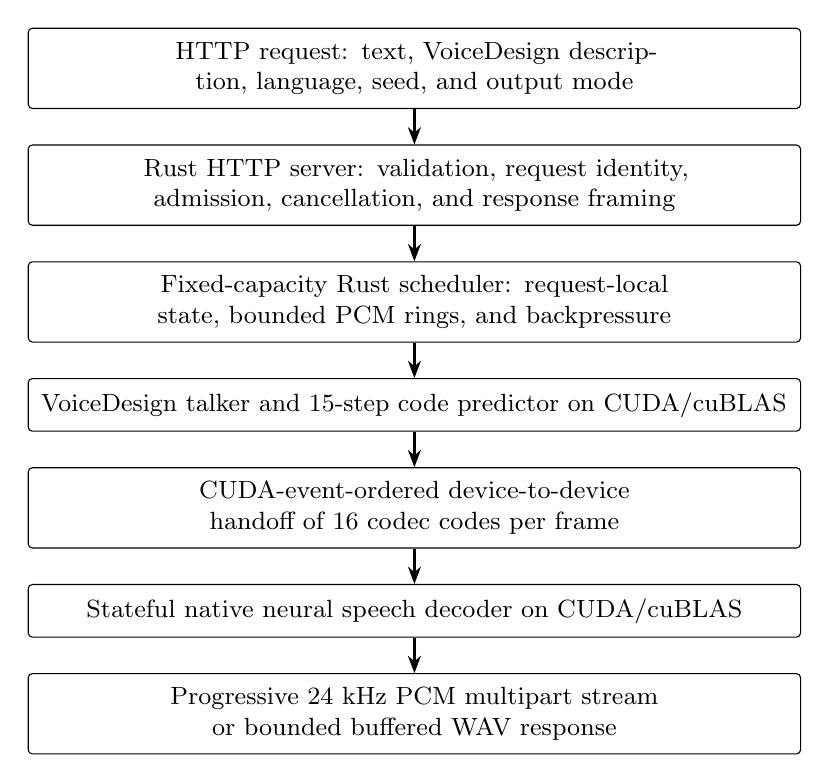
\begin{tikzpicture}[
  node distance=4.5mm,
  box/.style={
    draw=black,
    rounded corners=1.5pt,
    align=center,
    inner sep=5pt,
    text width=0.78\linewidth,
    font=\small
  },
  arrow/.style={-{Stealth[length=2.2mm]},thick}
]
  \node[box] (request) {HTTP request: text, VoiceDesign description, language, seed, and output mode};
  \node[box,below=of request] (server) {Rust HTTP server: validation, request identity, admission, cancellation, and response framing};
  \node[box,below=of server] (scheduler) {Fixed-capacity Rust scheduler: request-local state, bounded PCM rings, and backpressure};
  \node[box,below=of scheduler] (talker) {VoiceDesign talker and 15-step code predictor on CUDA/cuBLAS};
  \node[box,below=of talker] (handoff) {CUDA-event-ordered device-to-device handoff of 16 codec codes per frame};
  \node[box,below=of handoff] (decoder) {Stateful native neural speech decoder on CUDA/cuBLAS};
  \node[box,below=of decoder] (response) {Progressive 24 kHz PCM multipart stream or bounded buffered WAV response};

  \draw[arrow] (request) -- (server);
  \draw[arrow] (server) -- (scheduler);
  \draw[arrow] (scheduler) -- (talker);
  \draw[arrow] (talker) -- (handoff);
  \draw[arrow] (handoff) -- (decoder);
  \draw[arrow] (decoder) -- (response);
\end{tikzpicture}

  \caption{Implemented online path. Immutable model weights are shared, while
  mutable request state and CUDA execution resources are request-local. The
  diagram is a vector TikZ source and encodes no benchmark result.}
  \label{fig:architecture}
\end{figure}

Figure~\ref{fig:architecture} shows the complete online path. A single process
owns HTTP validation, scheduling, model execution, neural decoding, and
response delivery. The server loads one shared engine, creates a fixed-capacity
scheduler, and completes a real one-frame native warm-up before binding its
listener. Readiness therefore establishes that the model and end-to-end native
pipeline have produced a valid PCM packet; it is not merely a process-liveness
signal.

\subsection{Admission and ownership}

The canonical synthesis endpoint validates bounded JSON before attempting
engine admission. Text, textual VoiceDesign instruction, language, duration,
sampling settings, and response mode are checked at this boundary. Each
admitted request receives a unique identity and owns its cancellation state,
generation session, decoder session, CUDA stream and events, cuBLAS handle,
random state, PCM buffers, and scheduler slot. Immutable model weights are
shared across sessions.

The scheduler supports one through six active slots. Pending starts can be
coalesced for at most 2 ms, but capacity is fixed and exhaustion is explicit.
Each request has three reusable PCM buffers. A request advances only when a
buffer and queue position are available, so a slow client applies backpressure
instead of causing unbounded audio allocation.

\subsection{Packet cadence}

One codec frame represents 1,920 output samples, or 80 ms at 24 kHz. The first
decoder step requests one frame to minimize first-audio latency. Subsequent
steps request up to four frames and therefore produce at most 7,680 samples per
packet. This policy bounds buffering without forcing every later step to pay
the overhead of a one-frame packet.

\subsection{Lifecycle and failure handling}

Natural codec end-of-sequence closes a request after all owned PCM has been
delivered. Cancellation is propagated through the scheduler to native state,
and resource retirement is bounded. Model-contract, ABI, CUDA, packet-order,
and state-transition failures are surfaced instead of silently falling back to
a different implementation. The process does not attempt unsafe in-process
recovery of a stuck CUDA session.

\section{Native Implementation}

\subsection{Artifact boundary}

The runtime consumes the immutable VoiceDesign snapshot at revision
\code{5ecdb67327fd37bb2e042aab12ff7391903235d3}. Build-time and startup checks
validate configuration fields, tensor metadata, artifact hashes, and the
native ABI before serving traffic. The production image carries the
VoiceDesign weights and decoder-only speech-tokenizer material required for
inference. It excludes the tokenizer encoder, Base and CustomVoice checkpoints,
reference-audio functionality, and 0.6B weights.

\subsection{Talker and residual predictor}

The Rust model layer parses configuration and tokenizer artifacts, constructs
the VoiceDesign prompt from text, instruction, and official language name, and
owns the request lifecycle. Shared weights are uploaded once. Each session
retains independent key-value caches, workspaces, counters, random state, CUDA
stream, and cuBLAS handle.

For each codec frame, the talker predicts the semantic code and the native
15-step predictor produces the residual codebook values, yielding 16 codes per
frame. Sampling state is local to the request and is initialized from the
effective seed. Predictor and talker controls remain distinct; the predictor's
repetition penalty is fixed by the implemented model contract.

\subsection{Device-to-device handoff}

The production ABI avoids a codec-token round trip through host memory. The
talker exposes its device-resident frame and records a producer-ready CUDA
event. A non-blocking staging stream waits on that event, copies each frame into
a bounded device packet, and records completion. The decoder waits on the
packet-ready event and records a consumed event before the staging slot can be
reused. Tickets and device identity are checked so stale or cross-device state
cannot be accepted accidentally.

\subsection{Incremental decoder}

The decoder shares immutable weights but gives each active request its own
incremental neural state, stream, cuBLAS handle, events, histories, and bounded
PCM staging. CUDA kernels and cuBLAS execute the decoder path and clamp output
into signed 16-bit PCM. The current implementation uses non-blocking streams,
events, custom kernels, and cuBLAS. It does not claim CUDA Graph capture or
replay.

\subsection{Production image}

The runtime container targets \code{linux/arm64} and real \code{sm\_121} SASS
without a PTX fallback. The final stage contains CUDA runtime and the required
cuBLAS families but excludes compilers, development packages, Python, Node.js,
PyTorch, SGLang, vLLM, TensorRT, cuDNN, NPP, cuSPARSE, and NCCL. It runs as an
unprivileged user and is designed for a read-only root filesystem with dropped
Linux capabilities.

\section{Streaming API}

The primary endpoint is
\code{POST /v1/voice-design/speech}. A request contains non-empty UTF-8 text, a
natural-language VoiceDesign description, an optional language (default
\code{auto}), an optional seed, a bounded maximum duration, and an output mode.
The endpoint accepts VoiceDesign instructions only; a voice name, speaker
embedding, reference sample, or cloning identifier is not part of the schema.

Progressive responses use \code{multipart/mixed}. The first part is a JSON
start event, subsequent binary parts contain 24,000-Hz mono signed 16-bit
little-endian PCM, and exactly one JSON end or error event terminates the
application stream. Multipart boundaries define application packets; HTTP/1.1
chunks or HTTP/2 DATA frames do not. Figure~\ref{fig:streaming-cadence}
illustrates the packet cadence: the first packet carries one 80-ms codec frame
to minimize first-audio latency, and subsequent packets carry up to four
frames. A separate buffered mode returns a bounded RIFF/WAVE object after
synthesis completes.

\begin{figure}[t]
  \centering
  \begin{tikzpicture}[
  font=\footnotesize,
  pkt/.style={draw=black!55, rounded corners=1.5pt, minimum height=8mm, anchor=west},
  firstpkt/.style={pkt, fill=papernavy!85},
  laterpkt/.style={pkt, fill=papernavy!20},
  jsonpkt/.style={pkt, fill=neutralfill, align=center, font=\scriptsize, inner xsep=3pt},
  lbl/.style={font=\scriptsize, align=center, black!70},
  brace/.style={decorate, decoration={brace, amplitude=4pt}, black!60, semithick}
]
  % Scale: 1 codec frame (80 ms of audio) = 6 mm.
  \node[jsonpkt] (start) at (0,0) {JSON\\start};
  \node[firstpkt, minimum width=6mm]  (p1) at ([xshift=2.5mm]start.east) {};
  \node[laterpkt, minimum width=24mm] (p2) at ([xshift=2.5mm]p1.east) {};
  \node[laterpkt, minimum width=24mm] (p3) at ([xshift=2.5mm]p2.east) {};
  \node[laterpkt, minimum width=24mm] (p4) at ([xshift=2.5mm]p3.east) {};
  \node[lbl, anchor=west] (cont) at ([xshift=2mm]p4.east) {$\cdots$};
  \node[jsonpkt] (end) at ([xshift=2mm]cont.east) {JSON\\end / error};

  % Staggered top annotations so the labels cannot collide.
  \draw[brace] ([yshift=1mm]p1.north west) -- ([yshift=1mm]p1.north east);
  \node[lbl, anchor=south east, xshift=-2mm] at ([yshift=3.2mm]p1.north)
    {first packet: 1 frame\\= 80 ms audio};
  \draw[brace] ([yshift=1mm]p2.north west) -- ([yshift=1mm]p4.north east)
    node[lbl, midway, above=5pt]
    {subsequent packets: up to 4 frames = 320 ms audio each};

  \draw[brace, decoration={brace, mirror, amplitude=4pt}]
    ([yshift=-1.5mm]start.south west) -- ([yshift=-1.5mm]end.south east)
    node[lbl, midway, below=6pt]
    {one \code{multipart/mixed} application stream; multipart boundaries define
     packets,\\ not HTTP/1.1 chunks or HTTP/2 DATA frames};

  \draw[-{Stealth[length=2.2mm]}, semithick, black!60]
    ([xshift=-1mm,yshift=-17mm]start.west) -- ([xshift=4mm,yshift=-17mm]end.east)
    node[lbl, pos=0.5, below=2pt] {time};
\end{tikzpicture}

  \caption{Progressive response layout. The stream is bracketed by JSON start
  and end events; binary packet widths are drawn proportional to the audio
  duration they carry (80~ms first, then up to 320~ms each). The figure
  encodes the framing contract only, not a measured timing.}
  \label{fig:streaming-cadence}
\end{figure}

The service also exposes liveness, readiness, capability discovery, bounded
request cancellation, and prompt-free Prometheus counters. A conservative
compatibility endpoint returns buffered WAV but is not presented as a complete
implementation of any third-party audio API.

The standalone process does not terminate TLS or implement identity. A public
deployment therefore requires an authenticated and rate-limited proxy with
bounded request and response timeouts. Normal service logs and metrics omit
text, voice descriptions, language values, request identifiers, and generated
audio; surrounding proxies and clients require their own payload-retention
controls.

\section{Evaluation Methodology}
\label{sec:evaluation}

The evaluation is a controlled comparison of the native release candidate and
the pinned stock SGLang-Omni comparator on one DGX Spark. It is designed to
answer serving-system questions about latency, throughput, streaming cadence,
resource use, and reliability. It does not evaluate perceptual speech quality.

\subsection{Subjects and workload}

The production matrix contains 12 runs: two implementations, concurrency
profiles B1, B3, and B6, and two rounds. Each run performs 24 unmeasured warm-up
requests followed by at least 200 successfully completed measured requests.
Only one subject may use CUDA during a run. Round one executes stock SGLang
before Native; round two reverses that order and executes Native before stock
SGLang. The Native blocks on either side of the round boundary remain
consecutive, avoiding one unnecessary model reload while preserving the
required round-level order reversal.

Both subjects receive the exact same ordered JSONL workload, model repository
and revision, language, text, VoiceDesign description, seed, portable sampling
controls, streaming mode, and 20.48-s duration ceiling. Workload identity is
bound by SHA-256, including the ordered row seeds. The external Rust HTTP client
and localhost transport are shared.

Native completion is accepted only with explicit natural end-of-sequence,
\code{finish\_reason=stop}, and no length limit. The stock raw-PCM endpoint does
not expose a finish reason; its natural-EOS and length-limit fields must remain
unknown. As a conservative boundary gate, an accepted stock response must be
strictly shorter than 489,600 samples and 20.40 s. Passing that gate excludes a
known length-boundary case but does not prove natural EOS.

\subsection{Client-visible metrics}

The client records a monotonic start time immediately before writing each
request. Time to first audio (TTFA) ends when the first non-empty decoded PCM
payload byte reaches the client. Headers, multipart JSON, WAV headers, framing,
and zero-length transport chunks do not count as audio.

For request $i$, with wall time $w_i$ and decoded audio duration $a_i$,

\begin{equation}
  \mathrm{RTF}_i = \frac{w_i}{a_i}.
\end{equation}

For a concurrent scenario with elapsed wall time $W$ and successful requests
$S$, the throughput-oriented aggregate real-time factor is

\begin{equation}
  \mathrm{RTF}_{\mathrm{aggregate}} =
  \frac{W}{\sum_{i \in S} a_i}.
\end{equation}

The report keeps this quantity distinct from
$\sum_i w_i / \sum_i a_i$, which is a summed-request-wall latency view. It also
reports successful and attempted request throughput, first-to-final PCM
streaming window, packet arrivals, inter-packet gaps, response validity,
timeouts, cancellations, malformed responses, and explicit termination fields.

\subsection{Resource and energy measurement}

Timestamped host, cgroup, NVIDIA, and power telemetry is sampled every 100 ms;
a run fails if any required stream has an observed gap greater than 200 ms.
Measured-phase boundaries exclude warm-up work from performance and energy
reduction. Process RSS and GPU-visible unified memory are reported separately
and are not summed as independent physical memory. Energy is integrated from
the timestamped board-power series after subtraction of a separately measured
idle baseline, then normalized per generated audio minute. An unavailable
sensor remains unavailable rather than becoming an estimate.

\subsection{Fail-closed publication gate}

A run is excluded if another CUDA process is present, evidence is missing or
digest-mismatched, the workload or normalized sampling differs between
subjects, the success minimum is not met, Native completion is not natural EOS,
Stock EOS is imputed, telemetry cadence fails, or the comparator contains an
undisclosed execution change. Setup failures remain in the audit trail but do
not enter distributions. Every accepted evidence path is relative to the
manifest root and bound by byte length and SHA-256.

\section{Results}
\label{sec:results}

\ifFinalEvidenceAvailable
  \VerifiedResultSummary
\else
  \EvidenceWarning
  \VerifiedResultSummary
\fi

\begin{table}[t]
  \centering
  \caption{Per-run performance results. TTFA is measured at the client-visible first non-empty PCM byte. Aggregate RTF is scenario wall time divided by successful generated-audio duration.}
  \label{tab:benchmark-results}
  \small
  \resizebox{\textwidth}{!}{%
    \begin{tabular}{llcccccc}
      \toprule
      Engine & Round & Profile & Concurrency & Successes & TTFA p50 (ms) & TTFA p95 (ms) & Aggregate RTF \\
      \midrule
      \BenchmarkResultRows
      \bottomrule
    \end{tabular}%
  }
\end{table}


\begin{figure}[t]
  \centering
  \ifFinalEvidenceAvailable
  \pgfplotsset{
    perfaxis/.style={
      width=\linewidth,
      height=5.6cm,
      xlabel={Concurrency},
      xtick={1,3,6},
      xmin=0.5, xmax=6.5,
      grid=major,
      grid style={draw=black!12, densely dotted},
      axis line style={black!60},
      legend style={
        draw=none, fill=none, font=\footnotesize,
        at={(0.5,-0.32)}, anchor=north, legend columns=2,
        /tikz/every even column/.append style={column sep=10pt}
      },
      tick label style={font=\footnotesize},
      label style={font=\small}
    },
    nativemarks/.style={
      only marks, papernavy, mark=*, mark size=2.4pt
    },
    stockmarks/.style={
      only marks, papervermilion, mark=square*,
      mark options={fill=white, draw=papervermilion, line width=0.8pt},
      mark size=2.4pt
    }
  }
  \begin{minipage}[t]{0.49\linewidth}
    \centering
    \begin{tikzpicture}
      \begin{semilogyaxis}[
        perfaxis,
        ylabel={TTFA p95 (ms)},
        ymin=50, ymax=6000,
        log ticks with fixed point
      ]
        \addplot[nativemarks]
          table[x=concurrency,y=ttfa_p95_ms] {data/native-runs.dat};
        \addlegendentry{Native}
        \addplot[stockmarks]
          table[x=concurrency,y=ttfa_p95_ms] {data/sglang-runs.dat};
        \addlegendentry{Stock SGLang}
      \end{semilogyaxis}
    \end{tikzpicture}
  \end{minipage}\hfill
  \begin{minipage}[t]{0.49\linewidth}
    \centering
    \begin{tikzpicture}
      \begin{axis}[
        perfaxis,
        ylabel={Aggregate RTF},
        ymin=0, ymax=1.1
      ]
        \addplot[nativemarks]
          table[x=concurrency,y=aggregate_rtf] {data/native-runs.dat};
        \addlegendentry{Native}
        \addplot[stockmarks]
          table[x=concurrency,y=aggregate_rtf] {data/sglang-runs.dat};
        \addlegendentry{Stock SGLang}
        \addplot[black!55, densely dotted, domain=0.5:6.5, samples=2] {1}
          node[pos=0.68, above=0.5pt, font=\scriptsize, black!55] {RTF = 1};
      \end{axis}
    \end{tikzpicture}
  \end{minipage}
\else
  \fbox{\parbox[c][4.5cm][c]{0.94\linewidth}{\centering
    \textbf{Validated benchmark plots pending}\\[6pt]
    The final vector panels are rendered only after all 12
    run records and their digest-bound evidence pass validation.}}
\fi

  \caption{Per-round client-visible TTFA p95 and aggregate real-time factor at
  concurrency 1, 3, and 6. Filled circles denote Native; open squares denote
  stock SGLang. The dotted RTF line marks real-time factor one. No interpolated
  or synthetic measurements are permitted.}
  \label{fig:performance-summary}
\end{figure}

\begin{table}[t]
  \centering
  \caption{Measured-phase resource and energy results. GPU-visible unified memory is reported separately from process RSS and is not added to it.}
  \label{tab:resource-results}
  \small
  \resizebox{\textwidth}{!}{%
    \begin{tabular}{llccccc}
      \toprule
      Engine & Round & Profile & Peak RSS (GiB) & GPU-visible memory (GiB) & Mean power (W) & Energy per audio minute (J) \\
      \midrule
      \ResourceResultRows
      \bottomrule
    \end{tabular}%
  }
\end{table}

\begin{table}[t]
  \centering
  \caption{Container and model footprint. Registry compressed size is
  reported only when digest-bound registry evidence exists; otherwise it is
  shown as N/A. Local unpacked size is never substituted for registry size.}
  \label{tab:container-results}
  \footnotesize
  \setlength{\tabcolsep}{5.5pt}
  \begin{tabular}{lrrrr}
    \toprule
    Engine & Local unpacked (GiB) & Registry compressed (GiB) & Model parameters & Model weights (GiB) \\
    \midrule
    \ContainerResultRows
    \bottomrule
  \end{tabular}
\end{table}


The final analysis must discuss both rounds, tails as well as central
tendencies, reliability counts, progressive versus completion-buffered
delivery, and any metric that fails to support a simple ranking. Aggregate RTF
under concurrency must not be replaced by mean per-request RTF. Memory claims
must preserve the distinction between host RSS and GPU-visible unified memory.
Image-size claims require registry evidence and must not substitute a local
unpacked Docker size for compressed transfer size.

\section{Limitations}

\label{sec:limitations}

The implementation and measurements target one platform:
\code{linux/arm64} on NVIDIA DGX Spark with \code{sm\_121}. They do not
establish portability or performance on x86-64, another GPU architecture, a
multi-GPU server, or a cloud accelerator. Two rounds on one host expose
run-to-run variation and reverse subject order, but they cannot characterize
population-level hardware variance or eliminate all persistent host-state and
thermal effects. Idle baselines and one-at-a-time CUDA isolation constrain
these effects without proving that they are absent.

The runtime supports only the pinned 1.7B, 12-Hz VoiceDesign checkpoint. It
does not implement voice cloning, reference-audio conditioning, speaker
enrollment, Base or CustomVoice checkpoints, or the 0.6B model. Explicit
language identifiers are limited to Chinese, English, Japanese, Korean,
German, French, Russian, Portuguese, Spanish, and Italian, plus automatic
selection. Unsupported languages are rejected rather than advertised from
anecdotal output.

The benchmark measures serving behavior, not speech naturalness,
intelligibility, instruction adherence, accent, or listener preference. A
faster result would not by itself demonstrate better audio. Conversely, the
same released checkpoint does not guarantee bit-identical waveforms across two
different implementations unless a separate parity test establishes that
property.

The native and stock HTTP paths do not expose identical termination semantics.
Native reports natural EOS explicitly; stock raw PCM does not. The evaluation
therefore preserves Stock EOS as unknown even when transport completion and a
conservative length gate succeed. Finally, the current native path does not use
CUDA Graph capture or replay, so this paper makes no claim about their effect.

\section{Reproducibility and Artifact Identity}

The release record binds source, containers, model material, workload, raw
measurements, telemetry, and rendered reports. Local Docker image IDs and
unpacked sizes are distinct from registry manifest digests and compressed
sizes; neither is inferred from the other. Native and stock model-artifact
inventories are also recorded independently even though both share the same
repository revision.

\begin{table}[t]
  \centering
  \caption{Digest-bound artifact identity. Every pending value must be replaced
  from the accepted production manifest before publication.}
  \label{tab:artifact-identity}
  \small
  \begin{tabularx}{\textwidth}{>{\raggedright\arraybackslash}p{0.31\textwidth}X}
    \toprule
    Record & Value \\
    \midrule
    Evidence state & \PaperEvidenceState \\
    Native Git commit & \NativeCommit \\
    Native local image ID & \NativeLocalImageId \\
    Native OCI digest & \NativeImageDigest \\
    Stock local image ID & \StockLocalImageId \\
    Stock OCI digest & \StockImageDigest \\
    Shared model revision & \code{5ecdb67327fd37bb2e042aab12ff7391903235d3} \\
    Native model-artifact SHA-256 & \NativeModelArtifactSha \\
    Stock model-artifact SHA-256 & \StockModelArtifactSha \\
    Evidence-manifest SHA-256 & \EvidenceManifestSha \\
    Evidence timestamp & \EvidenceTimestamp \\
    Evidence bundle & \EvidenceBundleUri \\
    \bottomrule
  \end{tabularx}
\end{table}

The intended public code location is
\url{https://github.com/luka-loehr/qwen3-tts-native}. At publication time, the
paper must point to an immutable release tag and OCI digest, not only to a
mutable branch. The release archive must contain the English LaTeX source,
bibliography, vector figures, generated plot data, final paper PDF, benchmark
report PDF, evidence manifest, and checksums. Large raw evidence may be hosted
separately when the repository cannot carry it, but the public URI and manifest
digest must remain stable.

Reproduction requires a clean pull by immutable image digest, an idle supported
GPU, the documented hardened run command, a successful full-pipeline readiness
check, and the external workload client. Reproducers should validate the
manifest before generating tables or plots and should report any hardware,
driver, power-mode, workload, or comparator difference rather than presenting
it as the original experiment.

\section{Ethics and Broader Impacts}

Description-conditioned speech can improve accessibility, multilingual
interfaces, educational tools, and local control over speech infrastructure.
It can also be used to create misleading or harassing audio. Removing
reference-audio cloning from this runtime narrows one misuse path but does not
make generated speech inherently benign: a textual description may still seek
to evoke a recognizable person, role, or demographic stereotype.

Deployers should require authorization, rate limits, abuse monitoring,
appropriate disclosure that audio is synthetic, and a retention policy for
input text and generated audio. Applications involving an identifiable person
require consent and applicable legal review. Provenance or watermarking should
be evaluated where the deployment context supports it; this runtime does not
claim to add an inaudible watermark.

Benchmark publication also has an integrity obligation. Failed trials,
contamination, unsupported languages, unknown EOS state, unavailable sensors,
and negative results must remain visible. Energy measurements from one device
should not be generalized into a lifecycle environmental claim without a
broader accounting boundary.

\section{Conclusion}

This paper describes a complete native Rust/CUDA serving path for the pinned
Qwen3-TTS 1.7B VoiceDesign checkpoint on NVIDIA DGX Spark. The system combines
request-local model sessions, event-ordered device token handoff, incremental
neural decoding, bounded scheduling, backpressure, cancellation, and
progressive PCM delivery in one process and one production image.

The accompanying evaluation design makes implementation comparisons auditable:
one external client, one ordered workload, two rounds, three concurrency
levels, explicit termination semantics, measured-phase telemetry, and
digest-bound raw evidence. Final performance, memory, energy, reliability, and
container-footprint conclusions will be stated only after the production
manifest validates and the evidence placeholders in this source have been
replaced.


\bibliographystyle{plain}
\bibliography{references}

\end{document}
